% required packages
\documentclass[MTech]{iitmdiss}
\usepackage[utf8]{inputenc}
\usepackage{titlesec}
\usepackage{times}
\usepackage{t1enc}
\usepackage{float}
\usepackage{amsmath,amsfonts,amssymb,amsthm, bm}
\usepackage{mathrsfs}
\usepackage[autostyle]{csquotes}
\usepackage{longtable}
\usepackage{amstext}
\usepackage{threeparttable}
\usepackage{textcomp}
\usepackage{rotating}
\usepackage{lscape}
\usepackage{gensymb}
\usepackage{lipsum}
\usepackage{placeins}
\usepackage{graphicx}
\usepackage{epstopdf}
\usepackage{wrapfig}
\usepackage{tabularx}
\usepackage{multirow}
\usepackage{amsmath} % easier math formulae, align, subequations \ldots
\usepackage{makecell}
\usepackage{hhline}
\usepackage{cellspace}
\usepackage{enumitem}
\usepackage{mwe}
\usepackage{hyperref}
\hypersetup{
    % citecolor=blue,
    % colorlinks=true,
    linkcolor=blue,
    filecolor=blue,      
    urlcolor=blue
    }
\usepackage{indentfirst} % for indenting the start of the paragraph
\usepackage{natbib} % for bibliography
\usepackage{algorithm}
\usepackage{algpseudocode}
\usepackage{svg}
\usepackage{caption}
\usepackage[list=true,listformat=simple]{subcaption}
\usepackage{adjustbox}
\usepackage{ltablex} 
\usepackage{color}
\usepackage{framed}
\usepackage{array}
\usepackage{multirow}
\usepackage{geometry} % Page settings\usepackage{capt-of}
\usepackage{bm}
\usepackage{verbatim}
\usepackage{multicol}
\usepackage{siunitx}
\usepackage{nomencl}


%%%%%%%%%%%%%% to remove the space between the table of contents items
\usepackage{tocloft}
\renewcommand{\cfttoctitlefont}{\hspace*{\fill}\Large\bfseries}
\renewcommand{\cftaftertoctitle}{\hspace*{\fill}}
\renewcommand{\cftlottitlefont}{\hspace*{\fill}\Large\bfseries}
\renewcommand{\cftafterlottitle}{\hspace*{\fill}}
\renewcommand{\cftloftitlefont}{\hspace*{\fill}\Large\bfseries}
\renewcommand{\cftafterloftitle}{\hspace*{\fill}}

%%%%%%%%%%%%%%%%%%%%%%%%% document begin %%%%%%%%%%%%%%%%%%%%%%%%%%%%%%%%%%
\begin{document}
\begin{titlepage}
\newgeometry{left=5cm,bottom=0.1cm}
\centering

{\doublespacing \huge \bfseries Computation of hydrodynamic forces and motions for a vessel with low to moderate
forward speed and calculation of drift forces} % Title of the project
\\ [1.5cm]


\emph{\large Dual Degree Project Report } % Type of meeting
\\[1cm] 

\begin{minipage}{1\textwidth}
\begin{center} \large
Submitted by: \textbf{Visharad Jaydas Borsutkar} % Name of the student
\\
Guide: {\bf Dr. Abhilash Somayajula} \\
Roll no: {\bf NA18B102} % Registration number of the student
\end{center}
\end{minipage} 
\\[2cm]

\emph{\large in partial fulfillment of the requirements \\ for the award of the degree of }
\\ [2cm]


{\large \bf MASTER OF TECHNOLOGY}
\\[2cm]



\includegraphics[width=4cm]{photos/logo.pdf}


\vspace{0.5cm}
\begin{minipage}{1\textwidth}
\begin{center} \large
\textbf {DEPARTMENT OF OCEAN ENGINEERING \\
INDIAN INSTITUTE OF TECHNOLOGY, MADRAS} % Name of the department
\\[0.3cm]

\end{center}
\end{minipage} 

\vspace{1cm}
{\large \today}
\end{titlepage}

\newpage
\pagenumbering{roman}
\certificate

% \addcontentsline{toc}{chapter}{CERTIFICATE}

This is to certify that the thesis titled {\bf  Computation of hydrodynamic forces and motions 
for a vessel with low to moderate forward speed and calculation of drift force}, 
submitted by {\bf Visharad Jaydas Borsutkar}, to the
 {\bf Indian Institute of Technology, Madras}, for the award of the degree of 
 {\bf Dual Degree}, is a bona fide record of the research work done by him under my s
 upervision. The contents of this thesis, in whole or in parts, have not been submitted 
 to any other Institute or University for the award of any degree or diploma.
\\[3cm]


\begin{singlespacing}
    \hspace*{-0.25in}
    \parbox{2.5in}{
    \noindent {\bf Guide :}\\[0.25cm]
    \noindent Dr. Abhilash Somayajula \\ [0.15cm]
    \noindent Assistant Professor \\[0.15cm]
    \noindent Department of Ocean Engineering\\[0.15cm]
    \noindent IIT Madras, 600036
    } 
\end{singlespacing}
\\[2cm]


\noindent Place: Chennai, TamilNadu 600036\\
Date: 5 May 2023  

\newpage
\acknowledgements
Words cannot express my gratitude to my supervisor, {\bf Dr. Abhilash Somayajula}, 
without whom this would have been impossible. I am deeply indebted to him for 
his constant guidance and motivation which helped me grow professionally and 
personally. His mentorship is not limited to research, and I am also thankful 
to him for his encouragement and advise regarding graduate program applications.

I would also like to acknowledge {\bf Prof. Sriram V}, {\bf Prof. Deepak Kumar} and 
{\bf Prof. Abhilash Somayajula}, members of my dual degree project review commitee, for 
their input and suggestions that helped my work.

I am grateful to my friends Karni, Shivesh, Subodh, Darshan Premkumar, with whom I had countless
discussions in the initial phase of this project and incase of any concept clarification.
I am also thankful to {\bf Research Guild group} for allowing me participate in the research work
and research seminars that immensly helped for my DDP work.

Last but not the least, I would like to express gratitude to my family for 
their unconditional support throughout my entire study at IIT Madras.

\newpage
\abstract
Prediction of the dynamic motions of the ship is an essential aspect in the early stages of design as well as later during the service life of the ship. It is crucial to know the motion characteristics of the ship along the six degrees of freedom to operate it safely in adverse sea conditions. The growing number of large ships demands predicting their optimum performance with respect to travel time, fuel efficiency, and the safety of cargo and personnel in specified shipping routes. This can be achieved using efficient and easy-to-use numerical tools capable of predicting hydrodynamics loads on floating vessels with steady forward speed and solving their motion responses in various wave conditions. This project explains the implementation of a three-dimensional potential theory-based program in Python with the consideration of forward speed effects. The theoretical formulation, numerical implementation, and result comparisons are presented in this thesis.

As a part of this dual degree project, a frequency domain 3D panel-based program has been developed and extensively compared against the outputs of MDLHydroD software. KCS and KVLCC2 ship hull forms are analyzed and validated against the MDLHydro software developed by Dr. Amitava Guha. The comparison results are found to be in excellent agreement.

    
\noindent {\bf \large Keywords} : Potential theory, Laplace equation, Boundary element method ( BEM ), Hydrodynamic, Wave structure interaction, Multibody interaction, forward speed, drift force.

\newpage
\tableofcontents

\newpage
\listoftables
\addcontentsline{toc}{chapter}{LIST OF TABLES}

\newpage
\listoffigures
\addcontentsline{toc}{chapter}{LIST OF FIGURES}

\newpage
\chapter*{\centering ABBREVIATIONS}
\addcontentsline{toc}{chapter}{ABBREVIATIONS}
\vspace{0.5cm}
\begin{table}[h]
\centering
\setlength{\tabcolsep}{12pt}
\renewcommand{\arraystretch}{1.5} % Default value: 1
\begin{tabular}{ll}
    {\bf DftFrc} & Drift force \\
    {\bf FkFrc} & Froude Krylov force \\
    {\bf ScFrc} & Scattering force \\
    {\bf GCS} & Global coordinate system \\
    {\bf BCS} & Body coordinate system \\
    {\bf RAO} & Response amplitude operator \\
\end{tabular}
\end{table}

\newpage
\chapter*{\centering NOTATIONS}
\addcontentsline{toc}{chapter}{NOTATIONS}
\vspace{0.5cm}
\begin{table}[h]
\centering
\setlength{\tabcolsep}{12pt}
\renewcommand{\arraystretch}{1.5} % Default value: 1
\begin{tabular}{ll}
    $\boldsymbol{\phi_T}$   &    Total potential \\
    $\phi_I$ & Incident potential \\
    $\phi_D$ & Scattering potential \\
    $\phi_j$ & radiation potential in $j_{th}$ mode of motion \\
    $\vec{x}_s$ & location of Source \\
    $\omega_I$ & Incident wave frequency \\
    $\omega_e$ & Encountering wave frequency \\
    $U$ & Forward speed \\
    $g$ & acceleration due to gravity \\
    $\sigma$ & source strength \\
    $n_k$ & unit vector in $k_{th}$ direction \\
    $\beta$ & wave incident angle \\
    $dS$  & Panel surface area \\
    $\epsilon$ & perturbation parameter \\
    $\vec{T}^{(2)}$ & second order term \\
    $\eta_j$ & wave motion RAO for $j^{th}$ mode of motion \\
    $A_{ij}$ & Added mass in $j^{th}$ mode of motion due to oscillation along $k^{th}$ direction \\
    $B_{ij}$ & Radiation damping in $j^{th}$ mode of motion due to oscillation along $k^{th}$ direction \\
    $F_I^k$ & Froude krylov force for $k^{th}$ mode of motion \\
    $S_I^k$ & Scattering force for $k^{th}$ mode of motion 
\end{tabular}
\end{table}



\newpage
\pagenumbering{arabic}
\chapter{INTRODUCTION}

%%%%%%%%%%%%%%%%%%%%% Objective %%%%%%%%%%%%%%%%%%%%%%%%%%%%%%
\section{Objective}
This Dual Degree project aims to achieve two primary goals. The first objective is to calculate 
the motion characteristics and forces on a floating structure traveling at a low to moderate 
forward speed in regular waves for the frequency domain hydrodynamic analysis tool {\bf HydRA}. This computation is done by utilizing a 3D 
panel-based potential theory method that involves using an infinite-depth green function. 
The second objective is to compute the second-order forces i.e. mean drift force. 
The implementation is done by keeping in mind that this method can be used for single body case 
as well as for multibody case. Also, then the program's output is validated against 
the MDLHydroD software.

The thesis is structured in the following manner. The first chapter includes an introduction, 
the objectives of the project, the background and motivation, and a literature review. The second chapter provides an explanation of the 
mathematical problem setup and derivation. Chapter 3 illustrates the solution to the numerical 
mathematical problem. Chapter 4, elaborates on the calculation of wave 
forces and motions. Likewise, Chapter 5 describes 
the computation of drift force. In the last chapter, the project outcomes are compared with 
other software tools such as MDLHydroD and WAMIT6.


%%%%%%%%%%%%%%%%% Background and Motivation %%%%%%%%%%%%%%%%%%%%%%
\section{Background and Motivation}
A floating object is exposed to multiple forces, such as wind, currents, waves, and other 
environmental loads. The issue of sea-keeping involves the computation of hydrodynamic 
parameters and forces acting on a floating structure when it is in waves. To solve the 
problem of wave-body interaction, hydrodynamic forces are calculated using numerical 
methods and potential theory. These calculations can then be used to compute the RAOs 
(response amplitude operator)
of different types of vessels.

Hydrodynamic analysis software can help naval architects optimize and enhance the design of 
vessels in regular waves. It can provide insights into vessel's performance in various 
wave conditions, 
allowing designers to make informed decisions about the shape and size of the vessel. 
Moreover, it saves costs by reducing the need for expensive physical testing.
Software for hydrodynamic analysis can allow designers to iterate designs faster, 
as they can quickly simulate and evaluate the performance of different design configurations. 
This can help reduce the time-to-market for new vessels and increase productivity.

The primary goal of this project is to develop a flask-based web application named 'HydRA' 
capable of computing hydrodynamic properties such as Froude Krylov force, scattering force, 
RAO, radiation damping, and Added Mass for a vessel in zero and non-zero speed scenarios.
Also, the implementation of drift forces captures the effect of second-order forces in 
the deep sea. The main idea behind building an in-house web application is to have a 
solid foundation for a hydrodynamic analysis tool that can be further improved and 
extended toward more complex problems. The work outlined in the thesis 
closely adheres to the study presented in \citet{guha2015estimation} 
and \cite{guha2012development}.

%%%%%%%%%%%%%%%%%%%%%% Literature review %%%%%%%%%%%%%%%%%%%%%%%%%%%%%%
\section{Literature review}

During the initial phases of ship design, it is vital to have knowledge about the vessel's stability to ensure efficient and safe 
operation at sea. Evaluating hydrodynamic forces and motion features of the ship in regular 
waves is an essential factor for designing a stable and secure vessel. As computational power 
has become more accessible, computational fluid dynamics (CFD) has become more popular 
in solving problems related to the interaction between fluids and structures. 
Despite advancements in CFD, it is a still time consuming process to predict responses. Therefore, 
CFD may not be a practical option during the preliminary design stage. 
Since, CFD is not feasible during the early stages of design due to its time-consuming nature,
potential theory based methods are still widely used for designing floating structures like oil 
production platforms, offshore wind turbines, wave energy converters, etc.
The potential theory method has been advanced by the strip theory approach, 
which involves dividing a ship into multiple 2D strips along its length. 
By combining solutions to various two-dimensional problems, the three-dimensional 
hydrodynamics problem can be determined. Many researchers have contributed to the 
development of this approach which includes \cite{newman1979theory}, 
\cite{ogilvie1969rational}, \cite{beck1990documentation}, \cite{journee2001theoretical}, 
\cite{salvesen1970ship}. Beacause, the strip theory method assumes the bodies are slender, it was 
not suitable for analyzing ship structures and offshore stuctures which have a non-slender shape.
Therefore, a 3D panel based potential theory was developed. In this method, the floating vessel is
descritized or is a mesh of quadrilateral or triangular panels with different source strengths.

Tuck and Faltinsen 1970 \cite{salvesen1970ship} provides a detailed review of the theoretical 
and mathematical models used to predict the motion of ships in waves and the resulting sea 
loads acting on the hull, which is based on the pressure distribution around the hull and 
the wave-induced accelerations. The paper covers the effects of ship design parameters, 
wave steepness and frequency, and wave-induced motions on ship motions. It presents a 
mathematical model for calculating the sea loads acting on the hull. The paper then 
discusses the effect of ship design parameters, such as beam and draft, on ship motions 
and the influence of wave steepness and frequency.

The calculation of the Green function efficiently for frequency and time domain analyses has 
been a long-standing research area. \cite{newman1979theory} provides a comprehensive list of 
methods to compute both frequency domain and time domain Green functions efficiently. 
Similar work on the zero speed frequency domain Green function has also been reported 
by \cite{telste1986numerical}. It describes the theoretical background of the green 
function and the numerical method used to evaluate it.

The book \cite{liapis1986time} is considered very important book for studying dynamics of ships and
floating structures. The book focuses on the time-domain analysis of ship motions and provides 
an in-depth discussion of various methods for solving the differential equations of motion 
for ships in time-domain, including numerical and analytical methods. This book also explains about the
equations shown in the section \ref{sec:numerical_dis}.

\cite{guha2013development} and \cite{guha2015estimation} discuss developing and validating a 
frequency domain program that uses numerical methods for predicting the motion and hydrodynamic 
forces acting on floating bodies, specifically ships.

When a floating body is subjected to ocean waves, it experiences not only first-order forces 
(linear wave forces) but also second-order forces, which are nonlinear in nature. 
The second order forces are better known by their physical effects on a floating
body as the added resistance or the mean drift forces
Second order forces become important when wave induced motions are large. 
Primarily, mean drift forces are computed using two menthods:
(a) far field method and (b) near field method. 

Far field method was introduced by \cite{maruo1957excess} which is based on diffracted and radiated
wave energy and momentum flux at infinity.
The paper analyzes the experimental 
data of model tests and the calculations based on hydrodynamic theory to estimate the additional 
resistance or mean drift force on the ship due to wave-induced effects. The study indicates that the additional 
resistance is proportional to the square of the wave amplitude and frequency, which is 
consistent with the second-order wave theory.

Near field method was introduced by \cite{boese1970einfache} which is based on direct integration of 
pressure on submerged surface in short uses potential theory.
This paper, describes a simple method for calculating the increase in resistance of a ship in waves. 
The method involves calculating the wave drag of the ship at zero speed and then using a 
correction factor to account for the effect of waves on the ship's resistance.

\cite{faltinsen1980prediction},  \cite{pinkster1980low} talks about the derivation of the equations 
for mean drift forces and also about the second order wave theory. 
\cite{faltinsen1980prediction} presents a method to predict the added resistance or drift force 
and propulsion of a ship in a seaway. 
The method is based on the potential theory and takes into account the 
effects of wave-induced motions on the ship's performance. The paper provides a detailed 
description of the theoretical background and numerical implementation of the method using
the perturbation theory. 
Faltinsen also presents experimental results that validate the accuracy of the method. 
This paper is a significant contribution to the field of ship hydrodynamics, providing a 
reliable and practical approach to predicting ship performance in a seaway.
\cite{pinkster1980low} concludes that second-order wave forces can have a significant
effect on the motions and loads of floating structures and should be considered in the 
design of offshore structure.

This project documents the development of added feature i.e. to be able to perform analysis 
with the effect of forward speed for simple single body case as well as for complex multi-body
case for the "HydRA" tool being developed in the research guild group at IIT Madras. In addition to 
that theory about drift force and its solution is also discussed. 

\newpage
\chapter{MATHEMATICAL MODEL}
In this thesis, a ship moving with a steady speed of $U$ in deep water with regular 
waves of wave amplitude $A$ and incident frequency $w_I$ traveling at an angle 
$\beta$ relative to the surge direction of the ship is considered. To address the seakeeping
problem, potential flow techniques are commonly employed. With the advancements in computing power, 
it is now possible to use the three-dimensional panel based potential theory method to compute 
the wave load.

\section{Co-ordinate System}

In order to set up the mathematical model, two co-ordinate systems are defined; one of them is the 
Global co-ordinate system ( GCS ), whose origin is located at a calm water level. The other one is 
the Body seakeeping co-ordinate system ( BCS ), whose origin is located at the mid-ship on the 
intersection of the water line and centerline of the ship. It is further assumed that the $x$-axis 
of the GCS points towards the east direction, whereas the $x$-axis of BCS points towards the sway 
direction of the ship. Co-ordinates of points represented in GCS are expressed as 
$\boldsymbol{x^e} = (x^e, y^e, z^e)$ whereas for the points in BCS it is expressed as 
$\boldsymbol{x^s} = (x^s, y^s, z^s)$. Global co-ordinate system, i.e., GCS, 
denotes the inertial frame of reference. Body geometry and body parameters, 
such as the location of the vertical center of gravity and radii of gyration, 
are defined with respect to BSC.
The translating frame of reference, BCS allows the formulation of the vessel response in 
six degrees of freedom due to incident waves and steady current of speed $U$ in $-x$ direction 
which is equivalent to forward speed with respect to GCS. By assuming a small wave amplitude, 
a linear boundary value problem can be established to determine the velocity potential.
\section{Velocity potential}
Assuming that the fluid flow is inviscid, incompressible, and irrotational the total velocity potential at any point inside the fluid domain is given as :
\begin{equation}
    \boldsymbol{\Phi} (\vec{x}, t) = [\, -Ux + \phi_P(\vec{x})\,] + [\, \phi_I(\vec{x}, \beta, \omega_I) + \phi_S(\vec{x}, \beta, \omega_I) + \sum_{j=1}^{6}n_j\phi_j(\vec{x}, U, \omega_e) \,]\, e^{i w_e t}
\end{equation}
where, 
\begin{itemize}
    \item $\omega_I$ is the incident wave frequency.
    \item $\omega_e$ is the encountering wave frequency.
    \item $\phi_P(\vec{x})$ is the potential due to the perturbation of steady translation of stream.
    \item $\phi_I(\vec{x}, \beta, \omega_I)$ is the incident potential due to incident waves.
    \item $\phi_S(\vec{x}, \beta, \omega_I)$ is the scattering potential due to the reflected 
    waves from the body.
    \item $\phi_j(\vec{x}, U, \omega_e)$ is the radiation potential generated due to the
    motion of body in $j^{th}$ mode of motion.
\end{itemize}
In the above equation, the perturbation potential $\phi_P$ has a relatively insignificant 
effect on the total 
potential at low to moderate ship speed and so it is ignored to reduce the complexity 
of the problem. Hence, the final equation for velocity potential is given as :
\begin{equation}
    \label{eq:velocity_potential}
    \boldsymbol{\Phi} (\vec{x}, t) = -Ux + [\, \phi_I(\vec{x}, \beta, \omega_I) + \phi_S(\vec{x}, 
    \beta, \omega_I) + \sum_{j=1}^{6}n_j\phi_j(\vec{x}, U, \omega_e) \,]\, e^{i w_e t}
\end{equation}
In the above equation, $\omega_I$ is the 
frequency of the wave experienced by the vessel when it is stationary. According,
to the Doppler effect the actual frequency experienced by a body with steady speed is different 
from the incident frequency of the source. Hence, in this problem, $\omega_e$ is the frequency of 
the wave experienced by the vessel when it is moving with a 
certain steady speed $U$, which is expressed in terms of incident or normal wave 
frequency $\omega_I$ , forward speed $U$, and incident angle $\beta$ as :
\begin{equation}
    \label{eq:omega}
    \omega_e = \omega_I - \frac{\omega_I^2}{g}\,U\cos\beta
\end{equation}

%%%%%%%%%%%%%%%%%%%%%%%%%%%%%%% Governing equation %%%%%%%%%%%%%%%%%%%%%%%%%%%%%%%%%%%%%%%%%%%%%%
\section{Governing equation}
The governing equations of the fluid flow are the continuity equation ( conservation of mass ) 
and the Navier-stokes equation ( conservation of momentum ). Under the assumption of inviscid 
and irrotational flow, the Navier-stokers equations reduce to Laplace equation given as :
\begin{equation}
    \label{eq:laplace_eq}
    \nabla^2 \boldsymbol{\Phi} (\vec{x}, t) = 0
\end{equation}

\section{Boundary conditions}
\label{sec:Boundary condition}
In addition to the governing equation, the velocity potential satisfies the boundary 
conditions over the fluid boundaries. The total boundary surface $S$ comprises the 
free surface $S_F$, mean body surface $S_B$, bottom surface $S_Z$, and the radiation surface
 $S_\infty$ bounding the horizontal infinite fluid domain. The surfaces are shown in 
 Fig. \ref{fig:boundary_surfaces} below.
\begin{figure}[H]
	\centering
	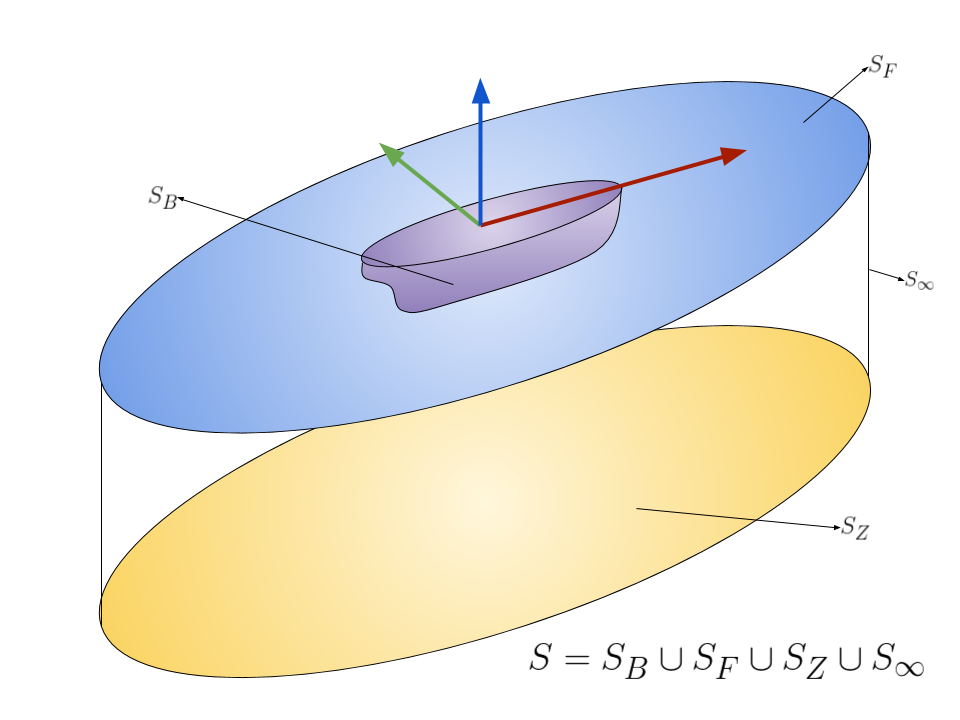
\includegraphics[width = 0.65\textwidth]{photos/boundary_surfaces.png}
	\caption{Fluid boundary surfaces}
	\label{fig:boundary_surfaces}
\end{figure}
The boundary conditions to be satisfied by the potential functions are shown below:

\begin{itemize}
    \item[1.] \underline{Kinematic free surface boundary condition} : 
    The velocity of the fluid in the direction normal to the free surface is equal to the velocity of the free surface. If the free surface is given by $z = \eta(t, x, y)$, then the boundary condition is given by
    \begin{equation}
        \label{eq:kin_free_surface_cond}
        \frac{\partial \eta}{\partial t} = \frac{\partial \phi}{\partial z} - \frac{\partial \phi}{\partial x} \frac{\partial \eta}{\partial x} - \frac{\partial \phi}{\partial y}\frac{\partial \eta}{\partial y} \quad \text{over} \; z
    \end{equation}
    
    \item[2.] \underline{Dynamic free surface boundary condition} : 
    The pressure on the free surface is constant and is obtained by the application of Bernoulli's 
    equation over the free surface.
    \begin{equation}
        \label{eq:dyn_free_surface_cond}
        \left[\left(i\omega_e - u\frac{\partial}{\partial x}\right) + g\frac{\partial}{\partial z}\right](\phi_I, \phi_D, \phi_j) = 0 \quad \text{on} \; z = 0
    \end{equation}
    
    \item[3.] \underline{Radiation boundary condition} :
    The waves generated by the oscillating body propagate outward from the body to $\infty$ in the fluid domain, unbounded horizontally. This boundary condition is also referred to as the Sommerfeld radiation condition.
    \begin{equation}
        \label{eq:sommerfel_rad_cond}
        \lim_{kr\rightarrow \infty}\sqrt{kr}\left(\frac{\partial}{\partial r} -jk\right)(\phi_j - \phi_I) = 0 \quad \text{for}\; i = 1, 2, \cdots 6
    \end{equation}
    
    % \newpage
    \item[4.] \underline{Bottom boundary condition} :
    The normal velocity of the fluid at the bottom boundary is equal to the normal velocity of the boundary. For an impenetrable seabed in deep water, the normal velocity is zero, and the boundary condition is given by 
    \begin{equation}
        \frac{\partial \phi}{\partial z} = 0 \quad \text{over the bottom}\; z = -\infty
    \end{equation}
    \item[5.] \underline{Body surface boundary condition}:
    The velocity of the fluid in the direction normal to the body boundary is equal to the normal velocity of the body boundary over the instantaneous underwater surface $S$.
    \begin{align}
        \label{eq:body_surface_boundary_cond}
        &\frac{\partial \phi_j}{\partial n} = i\omega_e n_j + Um_j \quad \text{on}\; S \\
        \label{eq:radiation_boundary}
        &\frac{\partial \phi_I}{\partial n} + \frac{\partial \phi_D}{\partial n} = 0 \quad \text{on}\; S
    \end{align}
\end{itemize}
\newpage
Here, $\vec{n} = (n_1, n_2, n_3)$ is the unit normal pointing outward from 
the hull surface and $(n_4, n_5, n_6)=\vec{r}\times \vec{n}$, where, $r$ 
is the position vector of a point on the surface. The linear incident wave 
potential satisfying the above boundary conditions is given by:
\begin{equation}
    \phi_I = \frac{igA}{\omega_I} e^{-ik_I(x\cos \beta + y\sin \beta)}e^{kz}
\end{equation}

 Here, $\omega_I$ represents the incident wave frequency, not the encounter frequency.
This forward speed boundary value problem can be solved using potential theory using 
infinite depth free surface green function. In general, free surface and body boundary conditions 
are non-linear and hence an exact solution is not possible. However, since the governing equation
is linear its solutions can be obtained by using perturbation approach.

\newpage
\chapter{NUMERICAL SOLUTION}
The complex potential on the submerged surface of the vessel is the key to solving the hydrodynamic problem. It will be shown that once the potential is known, all the hydrodynamic coefficients required to obtain all the vessel response, i.e., added mass, damping, and excitation forces, can be calculated.

The boundary value problem described in eq.(\ref{eq:kin_free_surface_cond}) to eq.(\ref{eq:body_surface_boundary_cond})  will be solved by a boundary element method. The body surface will be a suitable distribution of source singularities that satisfy the governing equation and the boundary conditions. Solving a Fredholm integral of the second kind over the discretized body boundary will determine the source strengths. 

%%%%%%%%%%%%%%%%%%%%%%%%%%%%%%%%%%%%%%%%%%%%%%%%%%%%%%%%%%%%%%%%%%%%%%%%%%%%%%%%%%%%%%%%%%%%%%
\section{Integral equation}
The velocity potential at some point $(x, y, z)$ in the fluid domain can be expressed in terms of the surface distribution of sources.

\begin{equation}
    \label{eq:vel_pot}
    \phi(\vec{x}) = \frac{1}{4\pi}\int_S \sigma(\vec{x_s})G(\vec{x}:\vec{x_s})\,dS
\end{equation}

where $\vec{x_s}$ denotes the source point of the body surface, $(\vec{x})$ denotes the point where the potential is being calculated, and $\sigma(\vec{x_s})$ is the unknown source strength distribution on the source point. Section (\ref{sec:green_fun}) will explain the Green function in the upcoming parts. 
The Green function satisfies the continuity condition and all the boundary conditions, including the free surface and radiation boundary condition, except for the following normal velocity boundary condition on the hull surface:

\begin{equation}
    \label{eq:vel_boundary_cond}
    \frac{\partial \phi}{\partial n} = v_n \quad \text{on}\; S
\end{equation}

Here, $v_n(x, y, x)$ is the flow normal velocity on the hull surface, after applying the velocity boundary condition given in equation (\ref{eq:velocity_potential}) on the velocity potential (\ref{eq:vel_pot}), the below equation is obtained, also known as Fredholm integral of the second kind.
\begin{equation}
    \label{eq:integral_eq}
    -\frac{1}{2}\sigma(\vec{x_s}) + \frac{1}{4\pi}\int_S\sigma(\vec{x_s})\frac{\partial G(\vec{x}:\vec{x_s})}{\partial n} = v_n \quad \text{on}\; S
\end{equation}
In the above equation, it can be shown that the first term reduces to $-\frac{\sigma}{2}$. Also, 
$\frac{\partial G}{\partial n}$ denotes the derivative of the Green function in the outward normal direction. This derivative of $G$ can be evaluated from the equation :
\begin{equation}
    \frac{\partial G}{\partial n} = \frac{\partial G}{\partial x}n_x + \frac{\partial G}{\partial y}n_y + \frac{\partial G}{\partial z}n_z
\end{equation}

\section{Numerical Discretization}
For $i^{th}$ panel eq.(\ref{eq:integral_eq}) can be written as:
\begin{equation}
    \label{eq:dis_integral_eq}
    -\frac{1}{2}\sigma_i(\vec{x_s}) + \frac{1}{4\pi}\int_S\sigma_i(\vec{x_s})\frac{\partial G_i(\vec{x}:\vec{x_s})}{\partial n} = v_{n_i} \quad \text{on}\; S
\end{equation}
Here, the subscript $i$ in the equation represents the entities of an individual panel.
While, calculating influence on a panel because of other source panel, the panel where the potential is being calculated and the source panel becomes the same. Due to this, frequency independant part of the green function tends to infinity. This case is known as singularity. To compensate for that influence, $-\frac{1}{2}\sigma$ is added into the equation according to the residual theory.

Eq. \ref{eq:dis_integral_eq} can be rearranged an written as:
\begin{equation}
    \label{eq:alpha_int_eq}
    -\frac{1}{2}\sigma_i + \frac{1}{2}\sum_{i=1, j=1, i\ne j}^{M}\alpha_{ij}\sigma_i = v_{n_i} \quad \text{for} i = 1, 2, \cdots M
\end{equation}
Here, $M$ is the total number of panels and $\alpha$ represents, 
\begin{equation}
    \label{eq:alpha}
    \alpha_{ij} = \frac{1}{2\pi}\int_{\Delta S_i}\frac{\partial G(x, x_s)}{\partial n} \,dS
\end{equation}
In physical terms, $\alpha_{ij}$ denotes the velocity induced at the $i^{th}$ panel in the direction normal to the surface by a source distribution of unit strength distributed uniformaly over the $j^{th}$ panel which is the source panel here and $i^{th}$ panel is the influenced panel where the potential is being calculated because of the presence of other source panels.

Now, the eq.(\ref{eq:alpha_int_eq}) can be written in the matrix format as :
\begin{equation}
    [\sigma] = 2[\alpha - I]^{-1}[v_n]
\end{equation}
where, $I$ represents the unit matrix. $[\alpha]$ is an $m\times m$ cross matrix where $m$ is the total no. of panels. Using the similar adjustments as done in the eq.(\ref{eq:alpha_int_eq}), eq.(\ref{eq:vel_pot}) can be written as
\begin{equation}
    \phi_i = \sum_{j=1}^{m}\beta_{ij}\sigma_{j}
\end{equation}
All potentials are computed at the centroid of the panels. Now, the above equation can be written in the matrix form as :
\begin{equation}
    \{\phi\} = [\beta]\{\sigma\}
\end{equation}
where, $[\beta]$ is the $M\times M$ matrix given by
\begin{equation}
    \label{eq:beta_eq}
    \beta_{ij} = \frac{1}{4\pi}\int_{\Delta S_j}G(\Vec{x_i}, \vec{x_s}) dS  
\end{equation}
Thus, the boundary problem can be solved for the velocity potential on the body surface if the value of the integral of the Green function $G$ and its derivatives $\frac{\partial G}{\partial n}$ are known.
%%%%%%%%%%%%%%%%%%%%%%%%%%%%%%%%%%%%%%%%%%%%%%%%%%%%%%%%%%%%%%%%%%%%%%%%%%%%%%%%%%%%%%%%%%%%
\section{Green's Function}
\label{sec:green_fun}
For the calculation of radiation and diffraction potential, an infinite-depth green function is used. This Green function and its numerical solution is explained in \cite{telste1986numerical}. 

This green function assumes source distribution over the submerged surface of the vessel. It relates the unknown source strength to the velocity potential. Here, the green function comprises two parts: one is the frequency-dependent part, and the other is the frequency-dependent part.  The Independent part represents the simple potential and interaction between the body surface and the free surface. On the other hand, the dependent part is to comprise the oscillating potential due to the oscillating source.
The equation of the Green function is given as 
\begin{equation}
    \label{eq:green_eq}
    G(\vec{x}, \vec{x_s}, \omega_e) = \frac{1}{r} + \frac{1}{\acute{r}} + \Tilde{G}(\vec{x}, \vec{x_s}, \omega_e) 
\end{equation}
where, 
\begin{equation}
    r = ||\boldsymbol{x} - \boldsymbol{x_s}|| = \sqrt{(x-x_s)^2+(y-y_s)^2+(z-z_s)^2}
\end{equation}
represents the Eucledian distance between the field point $P(x, y, z)$ and source point $Q(x_s, y_s, z_s)$.

\begin{equation}
    r' = \sqrt{(x - \xi)^2 + (y - \eta)^2 + (z + \zeta)^2}   
\end{equation}
represents the Euclidean distance between the field point $P(x, y, z)$ and point $Q'(\xi, \eta, \zeta)$, which is the image of the source point in the waterplane $z=0$ and $\tilde{G}(\vec{x}, \vec{x_s}, \omega_e)$ represents the frequency domain part of the green function, also refree. Note that the frequency used here is the encounter frequency $\omega_e$, shown in the eq. (\ref{eq:omega})

Now, substituting eq.(\ref{eq:green_eq}) in the equations (\ref{eq:alpha}) and (\ref{eq:beta_eq}), gives the following equations for $\alpha$ and $\beta$ matrices :

\begin{equation}
    \alpha_{ij} = -\iint_{\Delta S_i} \frac{\partial}{\partial n}\left(\frac{1}{r}\right) dS - \frac{1}{2\pi}\iint_{\Delta S_j} \frac{\partial}{\partial n}\left(\frac{1}{r'}\right) dS
    - \frac{1}{2\pi}\iint_{\Delta S_i} \frac{\partial G}{\partial n}(x_i, x_j, \omega_e) dS
\end{equation}
Here, $j^{th}$ panel is the source panel and $i_th$ panel represents the feild point where potential is supposed to be calculated.

\begin{equation}
    \beta_{ij} = -\frac{1}{4\pi}\iint_{\Delta S_i}
\end{equation}

\subsection{Frequency independent part of Green function}

\subsection{Frequency dependent part of Green function}
\section{Wave Potentials}
\section{Exciting forces}
\section{Forward speed RAO}

\newpage
\chapter{Forces and motions}
\section{Wave Potentials}
\section{Exciting forces}
\section{Forward speed RAO}

\newpage
\chapter{DRIFT FORCES}
\section{Introduction}
Mean drift forces are the mean non-linear forces which can be obtained using perturbation theory. 
Forces explained and computed in the previous chapters
are first order forces. While solving boundary value problems to get the potential, pressure, forces, 
motions, etc. usually
second order terms are ignored in order to reduce the complexity of the problem and also the mangitude of
second order terms which are these mean forces is also very small. But when the actual responses are very high,
these second order mean forces become important. These forces are proportional to swuare of the wave height 
while the 
first order are proportional to the wave height. Primarily, mean drift forces are computed using two menthods:
(a) far feild method and (b) near field method.

This chapter deals with the mean drift force and moments acting on a stationary vessel in regular waves. This chapter
presents the complete derivation of the second order force on an arbitrary shaped body moving with a steady 
forward speed in regular waves using 3D panel based potential theory. Far field method introduced by
\cite{maruo1957excess} is based on the diffracted and radiated wave energy and momentum flux at infinity. Near feild
method introduced by \cite{boese1970einfache} uses direct hydrodynamic pressure integration over the wetted surface and 
is based on 3D panel based potential theory.

\section{Pertubation Expansions}
\label{sec:perturbation_exp}
Perturbation theory is used to obtain the approximation solution upto a certain accuracy. Solution or quantity is 
expressed as a power series using a small paramater known as perturbation parameter. perturbation expression
starts with an avarage solution.
For example, 
\begin{equation}
    A = A_0 + \epsilon A_1 + \epsilon^2 A_2 + \cdots
\end{equation}
where, $\epsilon$ is the perturbation paramter and $A_0$ is the avarage solution of $A$.

Now, Assuming small amplitute motion oscillations about mean position of the body, approximations can be obtain 
up to second order with respect to the wave amplitute. Perturbation expressions of quantities 
of interest using a small parameter $\epsilon$ of the order of the wave slope, are given below :

\begin{itemize}
    \item [1.] Expressions for velocity potential $\left(\phi = \phi_T\,e^{i\,w_e\,t}\right)$ :
    \begin{equation}
        \phi = \epsilon \phi^{(1)} + \epsilon^2 \phi^{(2)} + \cdots
    \end{equation}

    \item [2.] The free surface elevation $(\zeta)$ :
    \begin{equation}
        \zeta = \epsilon \zeta^{(1)} + \epsilon^2 \zeta^{(2)} + \cdots
    \end{equation}

    \item [3.] The relative wave elevation:
    \begin{equation}
        \zeta_r = \epsilon \zeta_r^{(1)} + \epsilon^2 \zeta_r^{(2)} + \cdots
    \end{equation}

    \item [4.] The vessel motions :
    \begin{equation}
        \vec{\eta}(t) = \epsilon \vec{\eta}^{(1)} + \epsilon^2 \vec{\eta}^{(1)} + \cdots
    \end{equation}
    where, $\vec{\eta}^{(1)} = (\eta_1, \eta_2, \eta_3, \eta_4, \eta_5, \eta_6)$ represents the first order surge, 
    sway, heave, roll, pitch and yaw motions respectively.

    \item [5.] The pressure field in the fluid :
    \begin{equation}
        \label{eq:per_perssure}
        p = p^{(0)} + \epsilon p^{(1)} + \epsilon^{2} {^{(2)}} + \cdots
    \end{equation}
\end{itemize}



\section{Pressure and Force derivations}


\subsection{Pressure derivation}
The pressure using Bernoullis equation is given as:
\begin{equation}
    p = \frac{1}{2}\rho\,U^2 - \rho\,\frac{\partial \phi_T}{\partial t} - \frac{1}{2}\rho |\nabla\phi_T|-\rho\,g\,z^2
\end{equation} 
After substituting the above expression in eq.(\ref{eq:per_perssure}), pressure quatities with respect 
to different orders of $\epsilon$ are given as 
\begin{equation}
    p^{(0)} = - \rho g(z_B + z_0)
\end{equation}
where, $(\vec{X_0}) = (X_0, Y_0, Z_0)$ is the location of body coordinate system origin with respect to the global 
coordinate system and $\vec{x_B}=(x_B, y_B, z_B)$ the location of the point where the quantiy is begin computed in the body coordinate
system.
First order expression for pressure is given as:
\begin{align}
    P^{(2)} &= -\rho\frac{\partial \phi^{(2)}}{\partial t} + \rho\,U\frac{\partial \phi^{(2)}}{\partial x} -\frac{\rho}{2}
    \left\{\left(\frac{\partial \phi^{(1)}}{\partial x}\right)^2 + \left(\frac{\partial \phi^{(1)}}{\partial y}\right)^2 + 
    \left(\frac{\partial \phi^{(1)}}{\partial z}\right)^2\right\} \\ \nonumber
    &-\rho\left\{x^{(1)}\cdot\nabla \left(\frac{\partial \phi^{(1)}}{\partial t} - U\frac{\partial \phi}{\partial x}\right)\right\}
    - \rho g z^{(2)}
\end{align}
where, $z^{(2)} = [\eta_4\eta_6 x_B + \eta_5\eta_6 y_B - \frac{1}{2}(\eta_4^2 + \eta_5^2)z_B]$. All the potentails and 
their derivatives are calculated at mean position.
\subsection{Relative wave elevation}
Relative wave elevation is the distance between the wave surface and the instantaneous waterline. To calculate the
relative wave elevation, first absolute wave elevation needs to be calculated along the waterline. The waterline is obtained 
by extracting the edges of the panels which are at the water surface. According to the dynamic free surface boundary 
condition the pressure at free surface is zero ( guage pressure ) i.e. at $\zeta=0$, $p=0$. Hence, 
\begin{align}
    p &= 0 \quad \text{at} \quad z=\zeta \\ \nonumber
    \rho g \zeta + \rho\frac{\partial \phi}{\partial t} - \rho U \frac{\partial \phi}{\partial x} &=0 \quad \text{on} \quad z=\zeta 
\end{align}
Therefore the above equation yeilds :
\begin{equation}
    \zeta^{(1)} = -\frac{1}{g}\left(i\omega_e \phi_T - U\frac{\partial \phi_T}{\partial x}\right) e^{i\,\omega_e\,t}
\end{equation}
The relative wave elevation is  then obtained by subtracting the total movement of the body in $z$-direction from the
absolute wave elevation.
\begin{equation}
    \zeta^{(1)}_r =\zeta^{(1)} - (\eta_3 - \eta_5x + \eta_4y)
\end{equation}
where, $(x, y)$ are the centroid of the waterline panels or the waterline element.


\subsection{Forces and moments}
The hydrodynamic force is given as 
\begin{equation}
    F_H = -\int_S P\,n_j\,ds \quad \quad j=1, 2,\cdots, 6
\end{equation}
Using the perturbation expansions, equations for force can be written as
\begin{equation}
    \label{eq:per_force}
    \vec{F} = -\left(\int_{S_0}ds+\int_{wl}\zeta_r dl\right)(p^{(0)} + \epsilon p^{(1)} +
    \epsilon^2 p^{(2)}) (\vec{n}^{(0)}+\epsilon(\vec{\theta}^{(0)} \times \vec{n}^{(0)})+\epsilon^2H\vec{n}^{(0)})
\end{equation} 
The waterline integral arises due to the condideration of the first order wetted surface 
area $S_1$ which is the additional instantaneous surface of the hull below water considering 
both wave elevation and the motion of the body.
\begin{equation}
    \int_{S_1}\cdots ds = \int_{wl} dl \int_{0}^{\zeta_r}\cdots \frac{dz}{\sqrt{1-n^2_3}}
\end{equation}

Here, $wl$ is the waterline of the ship, $\zeta_r$ is the relative wave elevation and $dz/\sqrt{1-n^2_3}$ is the inclined height for 
non-wall sided surface. Now, after expanding the above equation and separating the terms with 
$\epsilon$, $\epsilon^1$ and $\epsilon^2$ gives the zeroth, first and second order force respectively.
Now, after substituting relative wave elevation in the eq(\ref{eq:per_force}) and extracting terms corresponding
to $\epsilon^2$, second order force can be obtained whose equation is given below :
\begin{align}     
    F &= -\int_{wl}\frac{1}{2}\rho g (\zeta_r^{(1)})^2 \frac{\vec{\eta}^{(0)}}{\sqrt{1-\eta_3^2}} dl + 
    \int_{S_0}\rho\left(\frac{\partial \phi^{(2)}}{\partial t} - U\frac{\partial \phi^{(2)}}{\partial x}\right)\vec{\eta}^{(0)}ds \\ \nonumber
    &+ \int_{S_0} \frac{\rho}{2}\left\{\left(\frac{\partial \phi^{(1)}}{\partial x}\right)^2 + \left(\frac{\partial \phi^{(1)}}{\partial x}\right)^2
    + \left(\frac{\partial \phi^{(1)}}{\partial x}\right)^2\right\}\vec{\eta}^{(0)} \,ds \\ \nonumber
    &+\int_{S_0}i\omega_e\rho\left\{(\eta_1-\eta_6y_B+\eta_5z_B)\frac{\partial \phi^{(1)}}{\partial x} \right. \\ \nonumber
    &\left. +(\eta_2+\eta_6x_B-\eta_4z_B)\frac{\partial \phi^{(1)}}{\partial y} + (\eta_3-\eta_5x_B+\eta_4y_B)
    \frac{\partial \phi^{(1)}}{\partial z}\right\}\vec{\eta}^{(0)} \,ds \\ \nonumber
    &- \rho g A^{(0)}\left[\eta_4 \eta_6 x_{B,f} + \eta_5\eta_6 y_{B,f} + \frac{1}{2}(\eta_4^2+\eta_5^2)Z_0\right]\hat{k} \\ \nonumber
    &-\omega^2_e\{-\eta_2\eta_6m + \eta_4\eta_6m z_g -\eta_6\eta_6 m x_g + \eta_3 \eta_5 m + \eta_4\eta_5y_g
    - \eta_5\eta_5 m x_g\} \hat{i} \\ \nonumber
    &-\omega^2_e\{\eta_1\eta_6m + \eta_5\eta_6m z_g -\eta_6\eta_6 m y_g - \eta_3 \eta_4 m + \eta_4 \eta_4 m y_g
    + \eta_4 \eta_5 m x_g\} \hat{j} \\ \nonumber
    &-\omega^2_e\{-\eta_1\eta_5 m - \eta_5\eta_5m z_g +\eta_5\eta_6 m y_g + \eta_2 \eta_4 m - \eta_4 \eta_4 m z_g
    + \eta_4 \eta_6 m x_g\} \hat{k}
\end{align}

Similarly, the second order moment can be given as :
\begin{align}
    \vec{M}^{(2)} &= -\int_{wl}\frac{1}{2}\rho g (\zeta_r^{(1)})^2 (x_B\times \vec{n}^{(0)}) dl \\ \nonumber
    &+\rho\int_{S_0}\left(\frac{\partial \phi^{(2)}}{\partial t} - U\frac{\partial \phi^{(2)}}{\partial x}\right)
    (\vec{x_B}\times\vec{n}^{(0)})\,ds \\ \nonumber
    &+\frac{\rho}{2}\int_{S_0}\left\{\left(\frac{\partial \phi^{(1)}}{\partial x}\right)^2
    \left(\frac{\partial \phi^{(1)}}{\partial y}\right)^2 + \left(\frac{\partial \phi^{(1)}}{\partial z}\right)^2
    \right\}(\vec{x_B}\times\vec{n}^{(0)})\,ds \\ \nonumber
    &+i\omega_e\rho\int_{S_0}
    \left\{(\eta_1-\eta_6y_B+\eta_5z_B)\frac{\phi^{(1)}}{\partial x} \right. \\ \nonumber 
    &\left. + (\eta_2-\eta_6x_B-\eta_4z_B)\frac{\phi^{(1)}}{\partial y}\right. \\ \nonumber
    &\left. + (\eta_3-\eta_5x_B+\eta_4y_B)\frac{\phi^{(1)}}{\partial z}\right\}
    (\vec{x_B}\times \vec{n}^{(0)})\,ds \\ \nonumber
    &-\omega_e^2\{\eta_2\eta_4my_g-\eta_1\eta_6mz_g-\eta_4\eta_6I_{54}
    -eta_5\eta_6I_{55}-\eta_6\eta_6I_{56} \\ \nonumber
    &+\eta_3\eta_4mz_g-\eta_1\eta_5my_g+\eta_4\eta_5I_{64}+\eta_5\eta_5 I_{65}
    +\eta_5\eta_6 I_{66} \}\hat{i} \\ \nonumber
    &-\omega_e^2\{\eta_3\eta_5mz_g-\eta_2\eta_6mz_g+\eta_4\eta_6I_{44}+\eta_5\eta_6 I_{45}
    +\eta_6\eta_6I_{46}\\ \nonumber
    &+\eta_1\eta_5mx_g-\eta_2\eta_4mx_g-\eta_4\eta_4 I_{64}-\eta_4\eta_5 I_{65}-\eta_4\eta_6 I_{66}\} \hat{j} \\ \nonumber
    &-\omega_e^2\{\eta_1\eta_6mx_g-\eta_3\eta_5my_g-\eta_4\eta_5my_g-\eta_4\eta_5 I_{44}
    -\eta_5\eta_5 I_{45}-\eta_5\eta_6 I_{46} \\ \nonumber
    &+\eta_2\eta_6my_g-\eta_3\eta_4mx_g+\eta_4\eta_4 I_{54}+\eta_4\eta_4 I_{55}
    +\eta_4\eta_6 I_{56} \}\hat{k} \\ \nonumber
    &+\rho g \left[-V^{(0)}\eta_1\eta_6+V^{(0)}\eta_4\eta_5x_{CB}-V^{(0)}\eta_5\eta_6z_{CB}
    -\frac{1}{2}V^{(0)}(\eta_4^2-\eta_6^2)y_{CB} \right. \\ \nonumber
    &\left.-\eta_4\eta_6L_{12} -\eta_5\eta_6L^{22}-\frac{1}{2}(\eta_4^2+\eta_5^2)
    Z_0A^{(0)}y_f+\eta_5\eta_6V^{(0)}Z^{(0)}\right]\hat{i} \\ \nonumber
    &+\rho g \left[-V^{(0)}\eta_2\eta_6+V^{(0)}\eta_4\eta_6 z_{CB}+\frac{1}{2}V^{(0)} 
    (n\eta-5^2-\eta_6^2)x_{CB} \right. \\ \nonumber
    &\left. +\eta_4\eta_6 L_{11}+\eta_5\eta_6L_{12}+\frac{1}{2}(\eta_4^2+\eta_5^2)Z_0A^{(0)}x_f
    -\eta_4\eta_6 Z_0V^{(0)}\right]\hat{j} \\ \nonumber
    &+\rho g V^{(0)}(\eta_1\eta_4+\eta_2\eta_5+\eta_5\eta_6x_{CB}-\eta_4\eta_6y_{CB})\hat{k}
\end{align}

added mass 
RAOS - random angles - 90-270 and one angle all 6
added mass , radiation damping, exciting force - one angle all 6


\newpage
\chapter{RESULTS AND DISCUSSION}
something something
\section{forward speed}
\subsection{KCS vessel}
\subsection{KVLCC vessel}
\section{Drift force}
\subsection{KCS vessel}
\subsection{KVLCC vessel}
% \subsection{KVLCC vessel}

\newpage
\chapter{CONCLUSION}

A new numerical web-based frequency domain tool is developed to compute hydrodynamic force and motions with low to moderate forward speed. The effect of forward speed is included using the encountering frequency and the changing boundary conditions.

\newpage
\bibliography{reference}
\addcontentsline{toc}{chapter}{REFERENCE}

\end{document}
